\section{Results}
Things to show:
\begin{enumerate}
    \item Introduce datasets and metric(s)
    \begin{enumerate}
        \item Artificial dataset that breaks uniform sampling
        \item Benchmark dataset from ESA paper
        \item Geometric dataset that breaks lightweight coresets
    \end{enumerate}
    \item Running sensitivity sampling with kmeans++ does not scale with $k$ but fast-kmeans++ solution does
    \item Uniform sampling and lightweight coresets both don't work on simple toy datasets
    \item The size of the coreset seems to make a difference when performing sensitivity sampling but not as much
          when doing lightweight coreset and uniform
\end{enumerate}

\subsection{Experimental Setup}
\subsubsection{Metrics}

We analyze the coreset construction methods along two metrics -- quality and construction time.  Although measuring runtime is standard, predicting coreset
quality is a more difficult task. Specifically, it is unclear how to confirm that a subset of points satisfies the coreset property over all solutions. To this
end, the authors in \cite{chrisESA} suggested the following procedure:
\begin{enumerate}
    \item Construct a sample coreset $\Omega$
    \item Use $\Omega$ to produce a candidate solution $C$ for the clustering task
    \item Report $\max \left( \dfrac{Cost(P, C)}{Cost(\Omega, C)}, \dfrac{Cost(\Omega, C)}{Cost(P, C)} \right)$, where $P$ is the original dataset
\end{enumerate}
We refer to this metric as the \emph{coreset distortion}. Naturally, values that are consistently close to $1$ suggest that solutions on the coreset are equally
viable on the full dataset.

\begin{figure*}
\label{fig:lightweight_breaks}
\centering
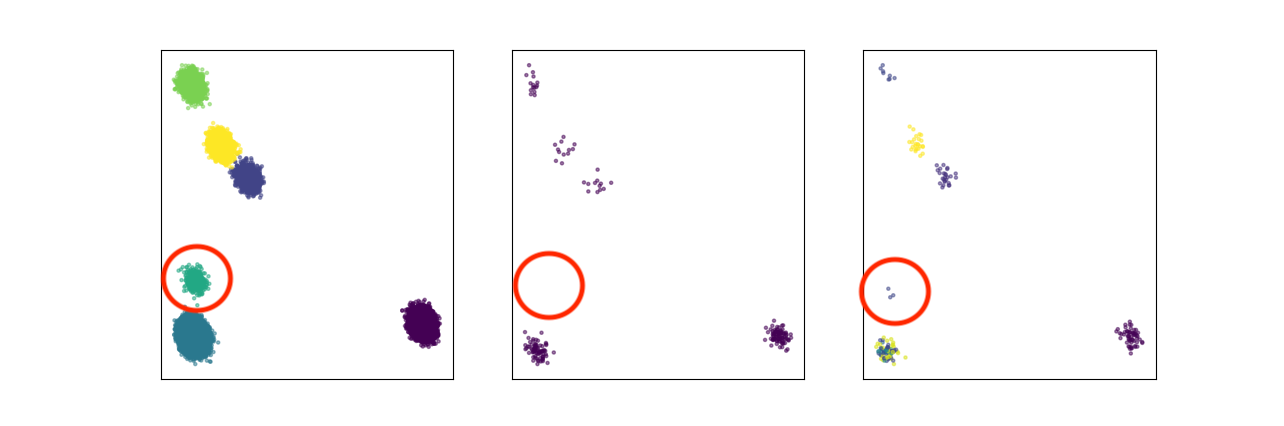
\includegraphics[width=.95\linewidth]{images/lightweight_breaks.png}
\caption{
The results of lightweight and fast-coreset constructions on a dataset of $n=100K$ points with clusters of varying size. Coresets have 200 points.
\emph{Left}: Original multivariate-Gaussian dataset. \emph{Middle}: Lightweight coresets fail to capture the cluster of $\sim$400 points.
\emph{Right}: The Fast-coreset construction runs in linear time but identifies all of the clusters.
}
\end{figure*}

\subsubsection{Algorithms}

We analyze five different algorithms for constructing coresets. The first is standard uniform sampling, where a subset of $m \ll n$ points are sampled from $P$.
Second, we incorporate the lightweight coreset construction discussed in \cite{lightweight_coresets}. There, we find the mean $\mu$ of the dataset and obtain
per-point sensitivity values that are proportional to $1/|P| + cost(p, \mu) / cost(P, \mu)$. The first term encourages uniform sampling while the second
encourages sampling proportionate to the distance from the mean.

The next two algorithms are the $k$-means++ and \fkmeans sensitivity sampling solutions, where we solve obtain an approximate $k$-means solution and
compute sensitivities using these preliminary centers.

We note that lightweight coresets are simply solving $1$-means to obtain sensitivity values whereas sensitivity sampling is solving the $k$-means problem.  As
we will show, it is easy to construct examples where lightweight coresets fail to produce acceptable coresets. Sensitivity-sampling, on the other hand, produces
satisfactory coresets across datasets and settings. The question then naturally arises: for what values of $j < k$ does an approximate $j$-means solution give
a satisfactory coreset? To this end, our last algorithm runs $j$-means++ for $j = f(k)$ where $0 < f(k) < k$ for all values of $k$. We default to $f(k) = \log
k$ but analyze other functions in \ref{ssec:alg_qualities}.

\subsubsection{Datasets}

We employ several real and artificial datasets to evaluate the quality of a coreset.  The artificial datasets are constructed to showcase specific weaknesses of
the various coreset construction algorithms. For example, consider that uniform sampling fails when each cluster has a different number of points. To this end,
the \emph{$1$-outlier} dataset, consisting of $n-1$ points in a single location and $1$ point placed at a large distance away, incurs arbitrarily bad distortion
under uniform sampling. 

Extending this, note that the lightweight coreset sensitivities are obtained by a linear combination of a uniform distribution and each point's relative
distance to the mean. As discussed, the uniform distribution can produce poor-quality coresets when presented with uneven class distributions. Furthermore, for
a zero-mean dataset, the relative distance to the mean is invariant to scaling while the coreset property is not. This means that one can obtain arbitrarily
bad lightweight coresets by taking a dataset with uneven class sizes, translating it to have zero-mean, and scaling all of the points by some $c >> 1$.

We demonstrate this through a \emph{Gaussian-mixture} dataset, comprised of multivariate Gaussians with varying cardinalities arranged randomly in
high-dimensional space. \textcolor{red}{Show plot or table of this}. We argue that this is a very realistic dataset to consider as there are many linearly
separable real-world datasets with imbalanced classes. Nonetheless, since the classes have different sizes and the means of the multivariate Gaussians are
normally distributed around the origin, the lightweight coreset algorithm fails to find a coreset of suitable quality. 

To measure the effect that the class imbalance has on the quality of lightweight coresets, we define a class imbalance parameter $\gamma$ and obtain each
cluster's size by $|C_i| = \frac{n}{m} \exp \left( \gamma(\rho - \frac{1}{2}) \right)$, where $\rho$ is distributed uniformly at random in the range $[0, 1]$.
Thus, $\gamma = 0$ means that each cluster has size $\frac{n}{m}$ and the cluster sizes vary as $\gamma$ grows. We see the effect of $\gamma$ on the coreset
distortion in Table \textcolor{red}{Table ref}, where even small values of $\gamma$ can break the lightweight coreset construction. Looking at the
$j$-sensitivities, we see that using $(j=\sqrt(k))$-means++ solutions maintains the coreset property for higher values of $\gamma$ but is still not guaranteed
to obtain satisfactory coresets. Despite this, sensitivity sampling consistently obtains coresets with low distortion.

As a harder example, we provide a \emph{geometric-progression} dataset, consisting of $n/2$ points at $(c, 0, 0, \cdots)$, $n/4$ points at $(0, c, 0, \cdots)$,
and so on. To see that this creates arbitrarily bad lightweight coresets as $c \rightarrow \infty$, consider that the likelihood of hitting each cluster goes to
zero if we only use a single center to estimate the sensitivities. We show furthermore that, for small values of $j$, sensitivities obtained
according to solving the ($j<k$)-means problem are insufficient to create a coreset for the geometric-progression dataset.

Lastly, we employ the \emph{Benchmark} dataset that was defined in \cite{chrisESA} as a particularly challenging problem for coreset constructions.  The
benchmark dataset is devised such that all reasonable solutions are of equal quality but maximally far apart in the solution space. This naturally stress-tests
the sensitivity sampling approach, as every candidate solution's sensitivities are particularly difficult to approximate.

For our real-world datasets, we utilize the MNIST, 1999 KDD-cup, Census, Cover Type, and song datasets \textcolor{red}{References}. \textcolor{red}{Write about the sizes}. In all real and
artificial datasets, we add random uniform noise $\eta$ with $0 \leq \eta_i \leq 0.001$ in each dimension so that the HST may separate the points into disjoint
cells.

\subsection{Algorithm Comparisons}
\label{ssec:alg_qualities}

We first verify the fact that coreset quality is independent of whether we used $k$-means++ or \fkmeans to obtain the preliminary solution. To this end,
Figure~\ref{fig:coreset_size_on_sens_quality} shows that, across datasets, the Fast-Coreset method produces coresets of consistent quality, with all distortion
values being lower than $1.2$. Additionally, for sufficient coreset sizes ($m \approx 80 * k$), Fast-Coresets are equal in quality to those obtained through
sensitivity sampling. Despite this, Figure~\ref{fig:k_on_runtime} shows that, while traditional sensitivity sampling runtimes grow linearly with $k$,
Fast-Coresets only grow logarithmically with the number of centers. Given this context, when reporting the sensitivity sampling results, we will be
specifically using the Fast-Coreset algorithm, with the knowledge that traditional sensitivity sampling would obtain slightly lower distortion and significantly
larger runtimes.

We now refer the reader to Figure~\ref{fig:coreset_size_on_quality}, where we show the effect of coreset size on the distortion across datasets and methods.
We define the coreset sizes as $|\Omega| = ck$, where $c \in [20, 40, 60, 80]$. We see that, across datasets, coresets of larger size obtain lower distortion. However
we also see that uniform, lightweight, and $j$-means coresets all fail on the geometric-progression and Gaussian-mixture datasets. Additionally, uniform
sampling clearly fails on the $1$-outlier dataset.

\begin{figure}
\centering
\begin{tabular}{lc}
    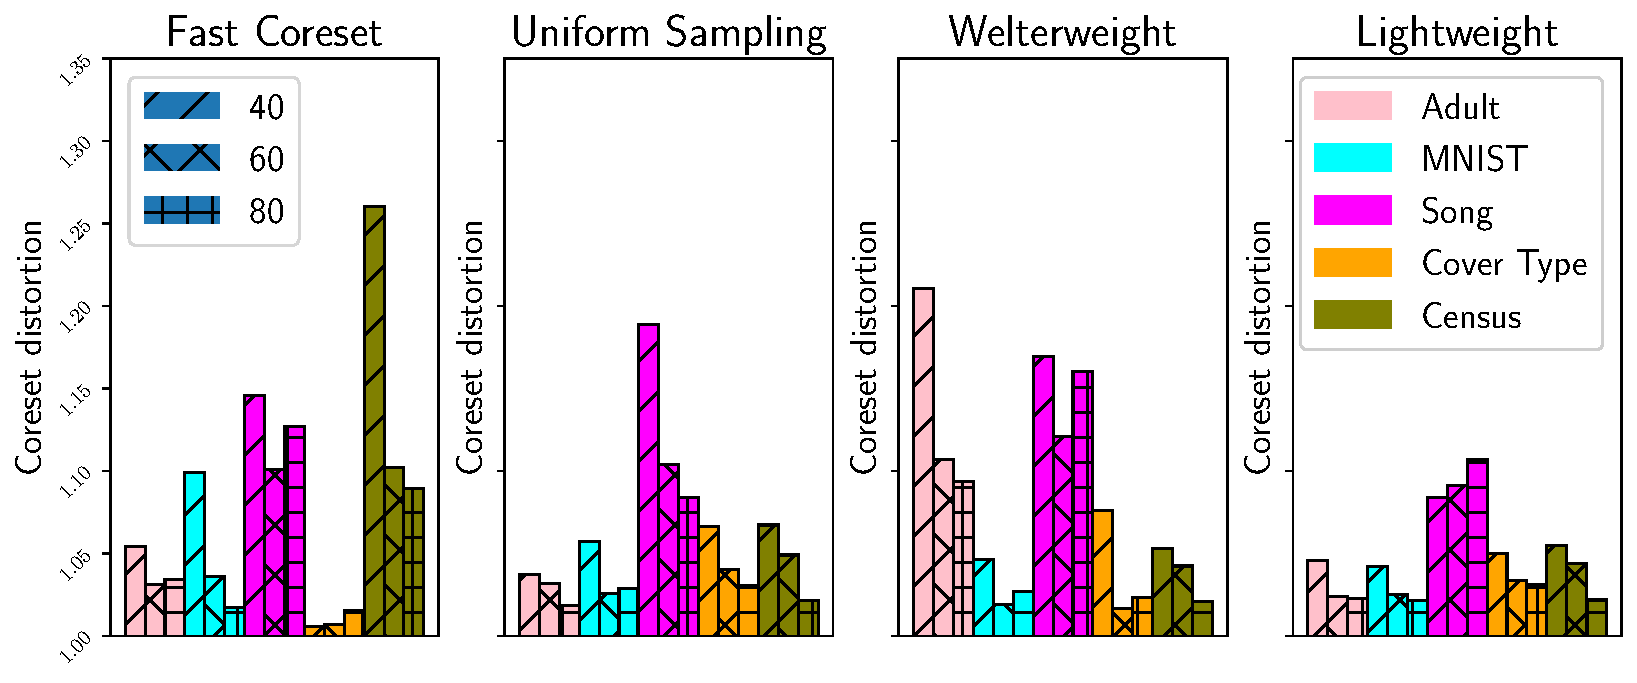
\includegraphics[width=\linewidth]{images/distortion_real_data} \\
    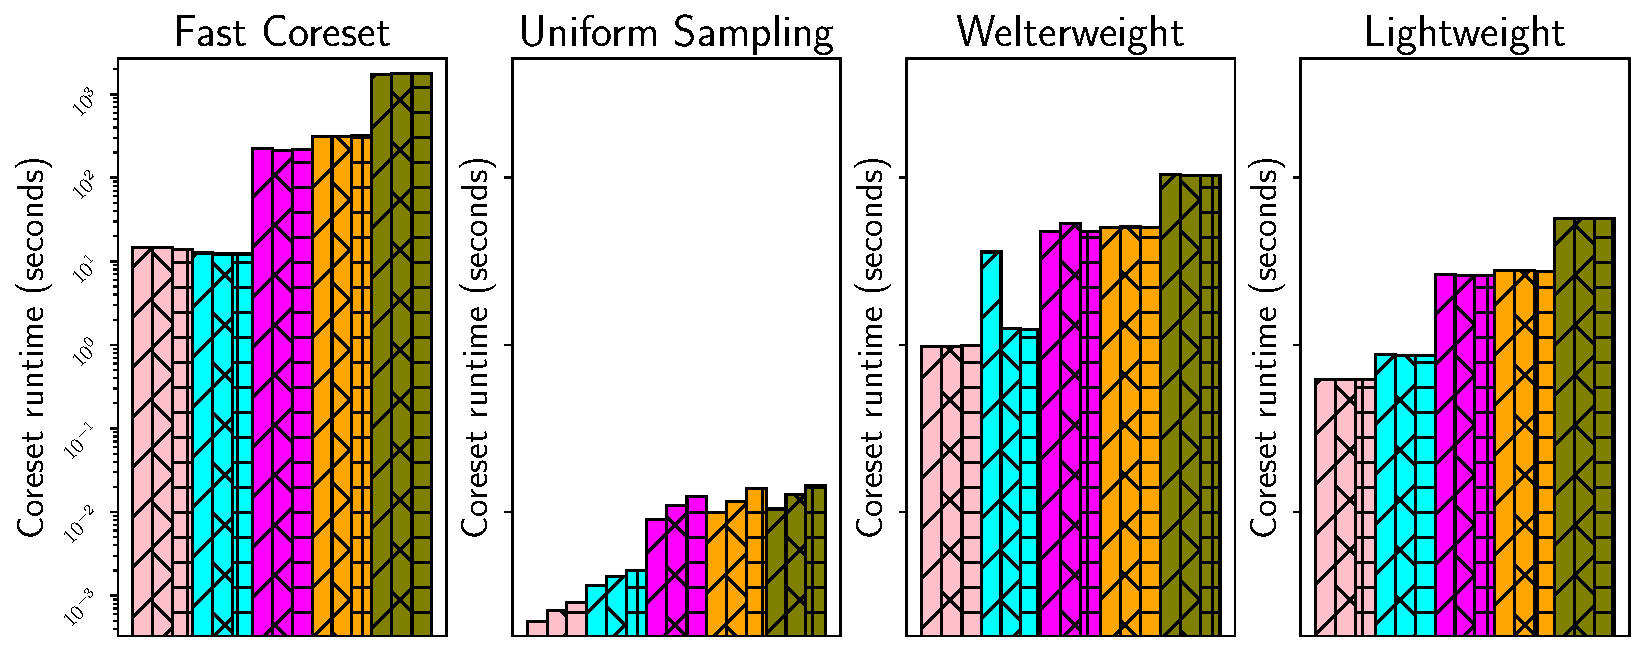
\includegraphics[width=\linewidth]{images/runtime_real_data}
\end{tabular}

\caption{\emph{Top}: The effect of the $m$-scalar on coreset distortion for real-world datasets. This is a visualization of the data in
Table~\ref{tbl:distortion}.  \emph{Bottom}: The effect of the $m$-scalar on the algorithm runtime for real-world datasets. All values are the mean over 5 runs.
The three bars represent samples of size $m=40k, 60k, 80k$.}

\label{fig:coreset_size_on_quality}
\end{figure}

\begin{figure*}
\label{fig:coreset_size_on_sens_quality}
\centering
\begin{tabular}{lc}
    \rotatebox[origin=l]{90}{\bf \;\quad\quad\quad\quad\quad\quad\quad$k$-Median} &
    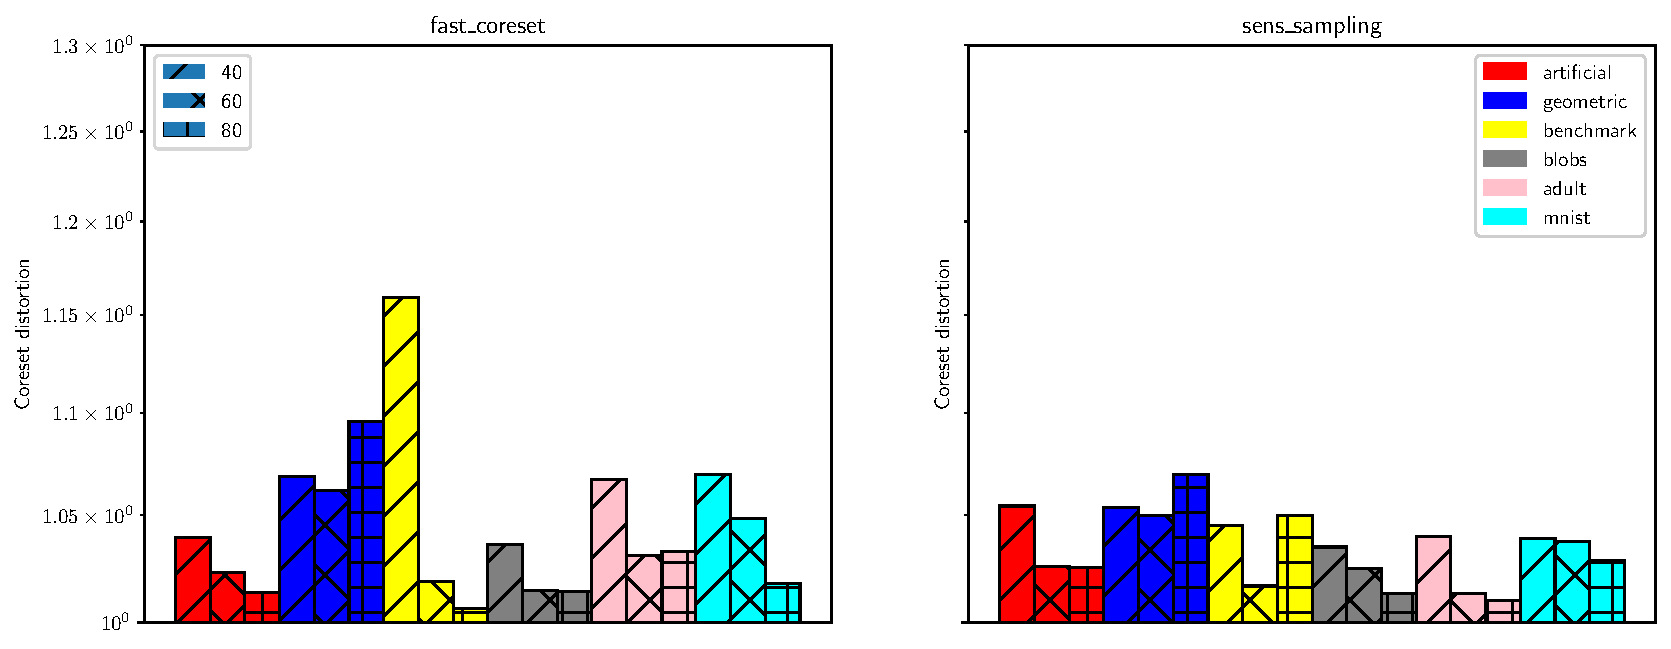
\includegraphics[width=.95\linewidth]{images/1/coreset_distortion-m_scalar_for_sens_sampling.pdf} \\

    \rotatebox[origin=l]{90}{\bf \;\;\quad\quad\quad\quad\quad\quad\quad$k$-Means} &
    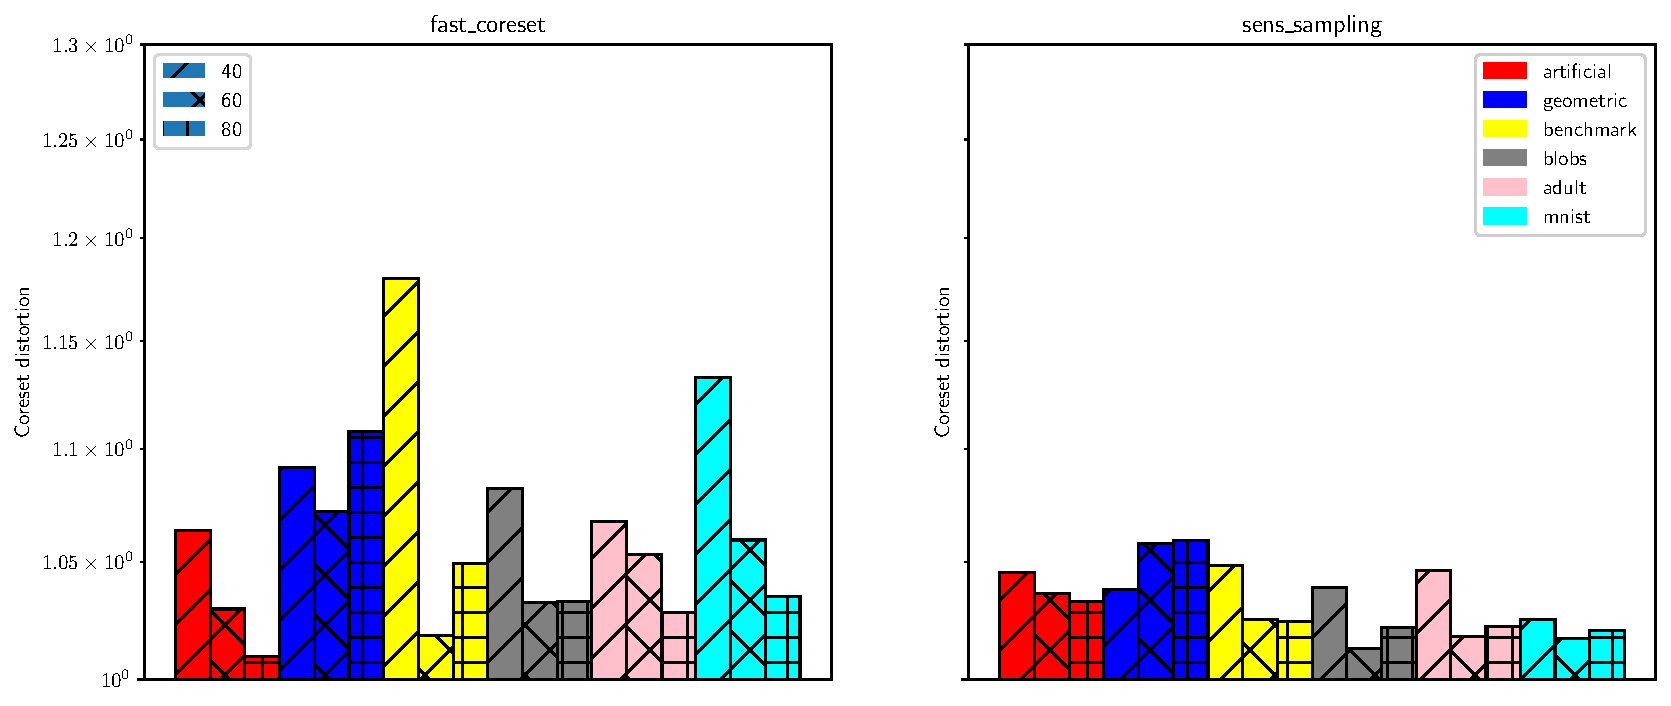
\includegraphics[width=.95\linewidth]{images/2/coreset_distortion-m_scalar_for_sens_sampling.pdf}
\end{tabular}
\caption{The effect of the coreset size on the distortion metric for sensitivity sampling approaches.
We point out that all distortion values are well below $\varepsilon = 0.2$.
Thus, for sufficient coreset sizes, there does not seem to be a meaningful difference between using Fast-Kmeans++ vs. regular Kmeans++.}
\end{figure*}

\begin{figure*}
    \centering
    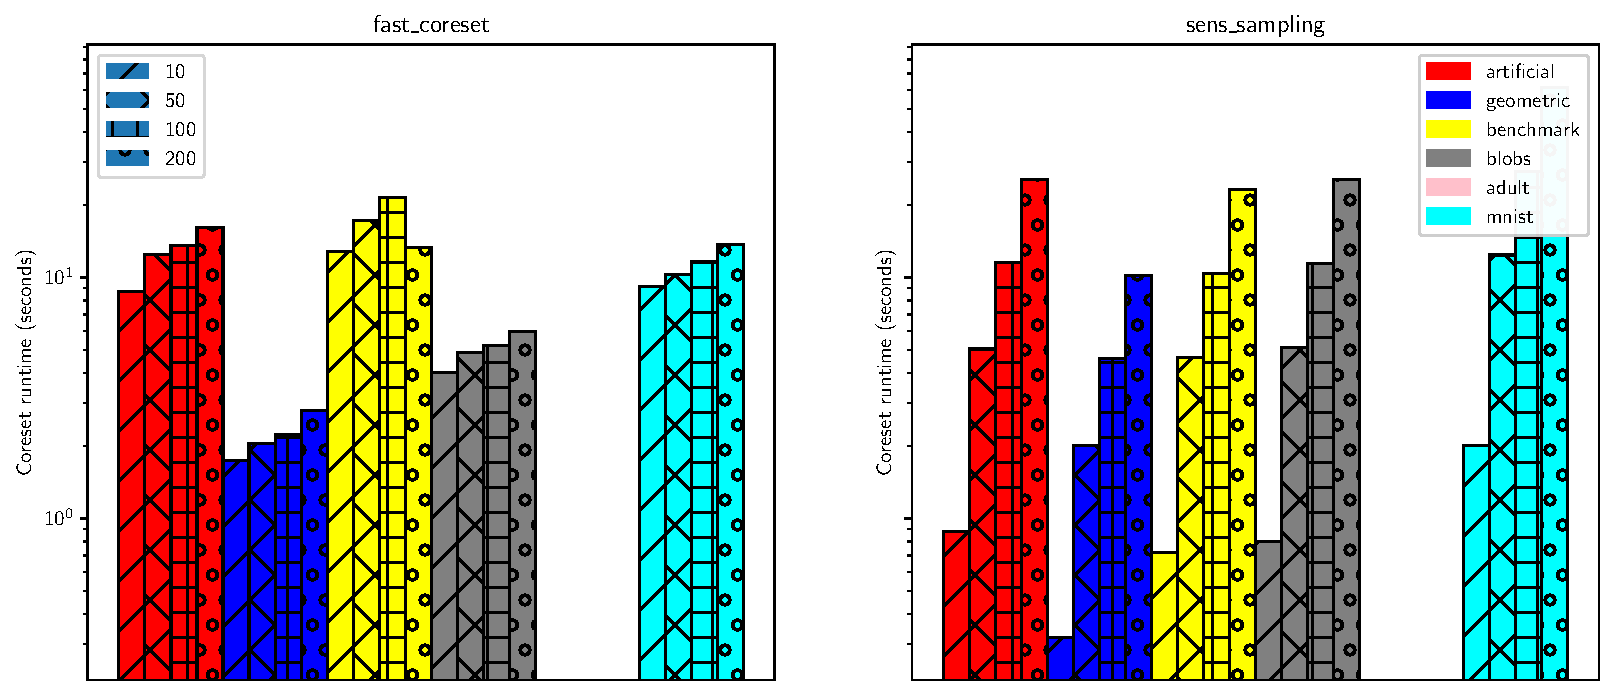
\includegraphics[width=.95\linewidth]{images/2/coreset_runtime-Effect_of_k_for_sens_sampling.pdf}
    \caption{
        The effect of $k$ on the coreset algorithm runtime. We see that traditional sensitivity sampling grows linearly with $k$ while Fast-Kmeans++ grows
        logarithmically.
    }
    \label{fig:k_on_runtime}
\end{figure*}

